\documentclass[a4paper,twocolumn,12pt]{article}

\usepackage[spanish]{babel}%formato de la fecha
\usepackage{flushend}
\usepackage[utf8]{inputenc} %tilde

% Elimina la indentación automática del comienzo de los párrafos
\setlength{\parindent}{0pt}

% Elimina la numeración de páginas
\pagestyle{empty}

% Configuración de fuente principal Times New Roman
\usepackage{times}
\usepackage{verbatim} 
\usepackage{graphicx}
\usepackage{hyperref}
\usepackage[
backend=biber,
sorting=ynt
]{biblatex}
\renewcommand{\section}[2]{}
\bibliography{biblio}

% Separación entre columnas de 1cm
\setlength{\columnsep}{1cm}

% Comandos personalizados
% =======================
% Fuente de tamaño 10: "{\chico TEXTO}"
\newcommand{\chico}{\fontsize{10pt}{5em}\selectfont}
% Fuente de tamaño 16: "{\grande TEXTO}"
\newcommand{\grande}{\fontsize{16pt}{5em}\selectfont}
% Todo lo que sea en tamaño 12, se escribe sin ninguno de estos comandos, ya que es el tamaño por defecto del documento

% Configuración de página A4 y márgenes de 2,5cm
\usepackage{geometry}
\geometry{
    a4paper,
    left=25mm,
    right=25mm,
    top=25mm,
    bottom=25mm,
}

% Autores
% Versión ciega, va sin autores!
%\author{Canizo, Franco Nicolás \\ 
%Manganiello, Michael Jonathan \\
%Morales, Yanina Graciela\\
%Terreno, Milton Ivan}

%http://minisconlatex.blogspot.com.ar/2012/03/como-escribir-un-articulo-con-latex.html


\begin{document}

% Parte inicial, sin separación en columnas
\twocolumn[
    \begin{@twocolumnfalse}
    
    % Título
    \begin{center}
        {\grande \textbf{YesDoc: Asistente médico personal}}
        
        \vspace{5mm}
        
        \textbf{\textit{Universidad Tecnológica Nacional, Facultad Regional Mendoza}}
    \end{center}
    
    
\end{@twocolumnfalse}
]

{\chico \textbf{Abstract}}

{\chico
%"El abstract debería ser considerado como una miniversión del artículo" (Day 1991). Describe los objetivos del estudio, la metodología usada, los resultados principales del trabajo y sus conclusiones fundamentales. Un abstract tiene típicamente un único párrafo y menos de 250 palabras y debe "permitir a los lectores identificar el contenido básico del documento rápida y fielmente, con el fin de determinar la relevancia del mismo para sus intereses y, por tanto, para decidir si necesitan leer el documento en su totalidad" (definición del American National Standards Institute). Será escrito en fuente (Times New Roman, 10, cursiva).
%YesDoc plantea un cambio de paradigma en el área de la medicina, en la que las instituciones  gestionan la información de forma privada e independientemente entre sí; Por uno en el que el usuario es dueño de sus datos, permitiéndole hacer uso de sus estudios desde cualquier lugar gestionando los datos de todas aquellas instituciones donde participe. Para esto se prevé implementar un sistema que le permita cargar los análisis e información relacionada a la salud por el mismo y por parte de las instuciones para q de este modo pueda transmitírsela al médico y observar su evolución a través del uso de gráficas.
%-----propuesta------ % tiempos verbales TODO EN PRESENTE

Este trabajo presenta a \textit{YesDoc}, una aplicación de salud cuyo objetivo principal es empoderar a las personas en el cuidado de su salud, generando un rol participativo y de compromiso.
\textit{YesDoc} mejora la atención médica, tanto en un plano de atención como de prevención, cambiando el paradigma actual donde la información la gestiona el médico, por uno en que el usuario es el propietario capaz de gestionarla según sus necesidades.
\textit{YesDoc} unifica los datos médicos, situando al usuario como eje principal. Permite llevar la información a donde más la necesite y disminuye los tiempos inter-consulta, ya que ofrece una comunicación fluida médico-paciente a través de su plataforma.  %sacar entre otros *resuelve la problemática actual en salud relacionada con la dispersión debido a la estructura descentralizada, sistemas informáticos de salud no adecuados, incomodidad en el transporte de resultados y largos tiempos inter-consulta, entre otros. **me pareció seguir aclarando lo que hacemos y no criticar
Brinda la unificación, centralización y disposición de información relacionada con el bienestar y la salud, sin importar la ubicación.
Permite gestionar las autorizaciones hacia terceros expertos o responsables/comprometidos, y brinda la seguridad de que esta información no será manipulada por una persona fuera del entorno de confianza. 
Permite el ingreso ágil, simple e intuitivo, y la presentación resumida, siempre comprensible, de diversos tipos de datos como mediciones, estudios e imágenes entre otros.
%diagnósticos y enfermedades.
% En esta parte teníamos que hacer una especie de explicación del proyecto pero no usar términos técnicos que si vamos a usar en la sección elementos de Trabajo y Metodología. La propuesta está acá abajo comentada. REVISAR
El trabajo consiste en el desarrollo de una aplicación web puesta a disposición de cualquier persona, diseñada para presentar una vista óptima sobre un amplio rango de dispositivos electrónicos tales como tablets, notebooks, computadoras personales y dispositivos móviles.
%usados actualmente, como pueden ser tablets, notebooks, computadoras personales y dispositivos móviles.
Esta aplicación consume servicios web dispuestos como recursos, tanto para \textit{YesDoc} como para cualquier otra aplicación de salud que requiera su uso.
Para garantizar la interoperabilidad con otros sistemas de salud, se tienen en cuenta los estándares informáticos mundialmente utilizados en el campo de la salud.
%El trabajo consiste en el desarrollo de una aplicación que hace uso de una API con servicio REST para aplicaciones de salud.El trabajo incluye el desarrollo de una aplicación web RESPONSIVE que hace uso de dicha API y se pone a disposición para ser usada por cualquier persona a través de su computadora personal, tablet o dispositivo móvil. Emplea estándares usados mundialmente tanto para informática como nomenclatura médica, garantizando así la interoperabilidad con otros sistemas de salud.
% utilizando las mejores prácticas de diseño, adoptando estándares de salud y aplicando herramientas tecnológicas actuales y adecuadas en los campos de seguridad, intercambio, almacenamiento y procesamiento de datos(OCR), 
 % HL7, cie10, cda, entre otros, buscando garantizar así la interoperabilidad con otros sistemas de salud.
%YesDoc permitirá a toda persona la unificación y centralización de la totalidad de su información relacionada con el bienestar y la salud, poniéndola a disposición de la misma y de terceros autorizados por ella.
%Proporcionará el ingreso de diversos tipos de datos, mediciones y estudios que serán gestionados personalmente, presentando un medio de uso simple, ágil e intuitivo para alentar y facilitar su uso, tanto al cargar la información de salud personal como al visualizarla en forma gráfica.
%Se hará uso de estándares utilizados mundialmente en registros médicos y de cuidado de la salud (como HL7 y CIE10), para garantizar la interoperatibilidad y comunicación con otros sistemas de salud.
%En cuanto a disponibilidad, el objetivo es que la persona pueda hacer uso de esta aplicación desde cualquier lugar del mundo y en cualquier momento, a través de Internet, usando un dispositivo móvil o una PC.
%Otorgará al propietario de la información, la posibilidad de interactuar con los profesionales médicos de su preferencia, brindándole a ellos los permisos adecuados para realizar consultas, seguimientos, aportar comentarios y/o dar conclusiones según sus requerimientos.
%A través de diversas tecnologías de cifrado, brindará la discreción, confidencialidad y seguridad necesarias para que la información no pueda ser accedida por personas o empresas malintencionadas que deseen utilizarla basándose en sus propios intereses.
%A lo largo del artículo se desarrollaran las dificultades y herramientas necesarias para llevar adelante dicho proyecto.
}

\vspace{3mm}
{\chico \textbf{Palabras Clave}}

{\chico
%Las palabras Claves propuestas por el Autor, para la indexación del documento. Serán escritas en fuente (Times New Roman, 10).
salud, registro personal de salud, phr, carpeta de salud, paciente, api, rest, responsive. 
}

\vspace{3mm}
\textbf{Introducción}

%La introducción sirve para que los lectores entiendan el contexto en el que se ha originado el trabajo y deja claro cuál es el tema básico. Contiene una descripción clara y precisa del problema que se ha abordado, explica su relevancia, cita y resume brevemente los trabajos que definen el problema y describen soluciones anteriores, para contextualizar la que se propone. Será escrita en fuente (Times New Roman, 12).
La idea de este trabajo surgió de los problemas que genera tener información médica en un formato físico, como puede ser papel, para diferentes estudios o imágenes, ya que la probabilidad de extraviar esta información es alta.
El traslado de los mismos es incómodo, y ocurre que en muchas de las consultas en la que es útil contar con los estudios médicos realizados previamente, el paciente no ha concurrido con éstos. 
%modificar la palabra "avance" "plagado" "metimos de lleno-> investigar profundamente"
% cita http://www.hoy.es/v/20110511/regional/tres-cada-diez-consultas-20110511.html
Relevando la situación actual identificamos que el proceso de interacción paciente-médico que plantea la estructura de salud actual, fomenta consultas innecesarias.
Esto provoca que los médicos tengan agendas cargadas, pero poco productivas.

% cita http://www.ehealthreporter.com/es/noticia/verNoticia/3784/fragmentacion-de-los-sistemas-de-salud-un-fenomeno-no-deseado
Al investigar profundamente acerca de los sistemas de salud actuales, nos encontramos con que en la provincia de Mendoza no existen desarrollos acordes a las necesidades del usuario y, sobre todo, adecuados a los estándares de salud, siendo incapaces de permitir la interoperatibilidad.

En cuanto a lo que refiere al aspecto legal de la salud en nuestro país, no existen aún leyes que contemplen los problemas previamente enunciados, aunque se está trabajando en una reglamentación que acompañe la digitalización de la información de salud en Argentina.
%existen grupos de personas involucrados en la materia que trabajan para lograr
%Claramente el problema acá es ... ..."problema-conflicto"
Concluimos que la estructura y tecnología presentes no cubren la necesidad tanto de médicos como pacientes de contar con datos de salud históricos, unificados, completos y disponibles de acuerdo con las facilidades que brindan las tecnologías.
Las leyes, tanto en nuestro país como en el mundo, no han logrado abordar estos conflictos.
Por lo tanto, es imperioso encararlos desde otra perspectiva: la del \textbf{paciente}, quien es el principal interesado en su salud.

Un ejemplo de solución a este problema es la conocida historia clínica universal.
El Reino Unido plantea, como un plan del departamento de salud denominado ``Cuidado y Salud personalizado'', lograr la integración de los registros de paciente para 2020.
España, por otro lado, había planteado hace 9 años implantar una historia clínica electrónica universal incorporada en la tarjeta sanitaria para todos los usuarios del Sistema Nacional de Salud.

Sin embargo, lo que ocurre es que hoy estas soluciones se encuentran con el problema de la integración y las trabas del sistema legal de salud de los propios países.
Para enfrentar este problema y lograr un resumen histórico de salud de la persona, se encara la situación desde otra perspectiva, centrándonos en el paciente, dejando así de lado la burocracia de instituciones médicas y de los mismos médicos, y creando una herramienta que le permita al paciente controlar su salud, que lo empodere y fomente su participación activa.
Sirve además a los médicos, ya que pueden consultarla con los permisos correspondientes, y a las instituciones médicas para mostrar al paciente los datos médicos de su propiedad.

%quizás habría que hablar de google health y health vault



%Hoy en día el crecimiento del uso de portátiles y de teléfonos inteligentes  brinda la posibilidad de poder llevar gran cantidad de información a cualquier parte, ahorrando en papel, espacio y hasta en tiempo por estar todo en un mismo lugar, utilizando estas herramientas tecnológicas se desarrollará un sistema web responsive y una aplicación móvil para que el usuario pueda gestionar su información como más lo prefiera brindando, además, la posibilidad de la conexión entre diferentes institutos.

Como se observa, la tendencia es hacia la integración, pero el problema es que los sistemas no han tenido esto en cuenta.
Por esto, se desarrolla una aplicación fiel a los estándares mundialmente utilizados, permitiendo así la interoperabilidad con sistemas actuales, y con sistemas futuros que cumplan con los mismos.

Además de esta característica primordial, el sistema se basa también en otros cuatro pilares fundamentales:
   
\begin{enumerate}
    \item Disponibilidad total

        \textit{YesDoc} brinda a toda persona la unificación y centralización de la totalidad de su información relacionada con el bienestar y la salud, poniéndola a disposición de la misma y de terceros autorizados por ella en cualquier lugar del mundo.
        El paciente concurrirá a la institución de salud solo en los casos en los que actualmente se considera necesario, se evitarán consultas solo para llevar resultados, también que el paciente repita estudios de forma innecesaria.
        %estudios que incluso pueden presentarse nocivos para la salud del paciente.

    \item Universalidad

        YesDoc garantiza que, sin importar la institución a la que concurras para ser atendido, la información sobre la salud del paciente sigue una línea temporal precisa. Las instituciones médicas no solicitarán reiterativamente sus datos personales. %(idea de que elegis la institución y esta usa tus datos y garantizara la seguridad de los mismos)

    \item Interacción

        YesDoc establece un nuevo paradigma de comunicación paciente-médico, que lleva el control del lado del paciente en una primera etapa de comunicación y luego deja en manos del médico la decisión sobre como proceder con la misma. Además permite establecer relaciones de confianza con personas allegadas o a cargo. %(que al principio la persona establece los permisos para que el medico vea los datos y despues el medico puede decidir comunicar resultados a traves del sistema o hacerlo por algun motivo de forma personal)

    \item Confidencialidad

        YesDoc brinda la discreción y seguridad necesarias para que la información no pueda ser accedida por personas o empresas que no correspondan.
%        malintencionadas que deseen utilizarla basándose en sus propios intereses.
\end{enumerate}


%implementará una API que permita a las instituciones poder hacer uso de la información del paciente

\vspace{3mm}
\textbf{Elementos del Trabajo y metodología}

%Es la parte sustancial del trabajo, el lector debe comprender el método usado con tal detalle que le permita aplicarlo al mismo o a otro problema. Se desarrollan los conceptos explicando la metodología utilizada. Será escrito en fuente (Times New Roman, 12).
Para llevar adelante la aplicación será necesario utilizar:

\textbf{API REST}, ``Application Programming Interface, REpresentational State Transfer'', es un tipo de arquitectura de desarrollo web que se apoya totalmente en el estándar HTTP (``HyperText Transfer Protocol''). REST permite crear servicios y aplicaciones que pueden ser usadas por cualquier dispositivo o cliente que entienda HTTP, %por lo que es increíblemente más simple y convencional que otras alternativas //yo sacaría esto
brindando la posibilidad de que otras aplicaciones puedan comunicarse con el sistema. Para su diseño debemos tener en cuenta que lo que presenta una API REST a las aplicaciones son \textbf{recursos}, éstos pueden ser utilizados por la aplicación a través de \textbf{URIs} (``Identificador de Recurso Único''), esto es, las URIs representan los medios por los cuales podemos llegar a un determinado recurso desde un navegador. Por otro lado tenemos las \textbf{representaciones}, éstas determinan como manipular los recursos en una arquitectura API RESTful, en general representan parte del estado del recurso que es transferido entre cliente y servidor. Por último, nuestra API RESTful presenta \textbf{servicios}, estos indican que es lo que puede obtener una aplicación de nuestros recursos haciendo uso de los métodos que define el protocolo HTTP. Entonces, a modo de resumen y ejemplo, nuestra API presenta un recurso, digamos una persona, a través del método GET de HTTP brinda el servicio de entregar información de la persona como puede ser el nombre, dirección, edad entre otras, contenida en determinada representación, digamos JSON (``JavaScript Object Notation''). Para que una API sea considerada REST debe cumplir 6 restricciones \cite{wiki:rest}:
\begin{enumerate}

	\item Interfaz uniforme
    
	    	Usar los verbos HTTP como las acciones que vamos a tomar sobre los recursos.
        
    \item Sin estado
            Cada mensaje entre el cliente y el servidor es completamente descriptivo lo que hace que no sea necesario almacenar información entre mensajes.
            
    \item Cliente-Servidor
    
    		Se asume un funcionamiento en una arquitectura de sistemas desconectados.
            
    \item Cacheable
    
    		Las respuestas del servidor pueden ser almacenadas en una memoria temporal intermedia de forma explícita, implícita, o previa negociación.
            
    \item Sistema en capas
    		
            Existencia de software o hardware intermedio entre el cliente y el servidor.
            
    \item Código bajo demanda
    
    		Esta restricción, a diferencia de las primeras cinco, es opcional y establece que parte de la lógica alojada en el servidor puede extenderse al cliente para que éste sea quien la ejecute.
            
\end{enumerate}
%Otra característica importante es que un servicio REST no tiene estado (es stateless), lo que quiere decir que, entre dos llamadas cualesquiera, el servicio pierde todos sus datos dejando de recordar entre peticiones, toda la información que se requiere para mostrar la información que se solicita debe estar en la consulta por parte del cliente. Al no guardar estado, REST nos permite escalar mejor sin tener que preocuparnos de temas como el almacenamiento de variables de sesión e incluso, nos permite utilizar distintas tecnologías para servir determinadas partes o recursos de una misma API. // Ésto lo sacaría porque está explicado en las restricciones de REST.

\textbf{La arquitectura MVC},
(modelo–vista–controlador) es un patrón de arquitectura de software que separa los datos y la lógica de negocio de una aplicación de la interfaz de usuario y el módulo encargado de gestionar los eventos y las comunicaciones. Para ello se propone la construcción de tres componentes distintos que son el modelo, la vista y el controlador, es decir, por un lado define componentes para la representación de la información, y por otro lado para la interacción del usuario. Esto presenta ventajas en la reutilización de código y la separación de conceptos, lo que facilita tanto el desarrollo como el mantenimiento de las aplicaciones.\cite{wiki:mvc}

\textbf{Open Source}, es el término con el que se conoce al software distribuido y desarrollado libremente. Nuestro proyecto se adapta a esta corriente de desarrollo para aprovechar algunas de sus ventajas como: 

\begin{itemize}
\item Mejora de la calidad y la innovación.
\item Reducción de costos mediante el ahorro del pago de licencias.
\item Reducción de dependencias de fabricantes de software.
\end{itemize}

Entre las dependencias Open Source que utilizamos podemos destacar a AngularJS, Plantuml \cite{wiki:plantUML}, GIT y Flask. Ademas nuestro código se encuentra disponible en GitHub.com bajo el nombre de la organización \textbf{YesDoc}.


\textbf{GIT como herramienta de control de versionado} que nos permite el mantenimiento de versiones del código de forma eficiente y confiable, permitiéndonos llevar un registro histórico de los cambios realizados

\begin{comment}
    \begin{itemize}
        \item Necesita menos veces estar conectado a la red para hacer operaciones. Esto produce una mayor autonomía y una mayor rapidez.
        \item     Aunque se caiga el repositorio remoto la gente puede seguir trabajando
        \item     Al hacer los distintos repositorio una réplica local de la información de los repositorios remotos a los que se conectan, la información está muy replicada y por tanto el sistema tiene menos problemas en recuperarse si por ejemplo se quema la máquina que tiene el repositorio remoto. Por tanto hay menos necesidad de backups. Sin embargo, los backups siguen siendo necesarios para resolver situaciones en las que cierta información todavía no haya sido replicada.
        \item     Permite mantener repositorios centrales más limpios en el sentido de que un usuario puede decidir que ciertos cambios realizados por él en el repositorio local, no son relevantes para el resto de usuarios y por tanto no permite que esa información sea accesible de forma pública. Por ejemplo es muy útil se pueden tener versiones inestables o en proceso de codificación o también tags propios del usuario.
        \item     El servidor remoto requiere menos recursos que los que necesitaría un servidor centralizado ya que gran parte del trabajo lo realizan los repositorios locales.
        \item     Al ser los sistemas distribuidos más recientes que los sistemas centralizados, y al tener más flexibilidad por tener un repositorio local y otro/s remotos, estos sistemas han sido diseñados para hacer fácil el uso de ramas (creación, evolución y fusión) y poder aprovechar al máximo su potencial. Por ejemplo se pueden crear ramas en el repositorio remoto para corregir errores o crear funcionalidades nuevas. Pero también se pueden crear ramas en los repositorio locales para que los usuarios puedan hacer pruebas y dependiendo de los resultados fusionarlos con el desarrollo principal o no. Las ramas dan una gran flexibilidad en la forma de trabajo.
    \end{itemize}
\end{comment}

\textbf{UML}, `` Unified Modeling Language'' es un lenguaje gráfico para visualizar, especificar, construir y documentar un sistema, este lenguaje nos guiará a lo largo del desarrollo para poder comprender el funciones del sistema desde distintas perspectivas y poder documentarlo en sus totalidad. Para poder explotar UML utilizaremos los siguiente diagramas que nos muestran diferentes aspectos.
  \begin{itemize}
    %\item Diagrama de caso de uso: expone las interacciones entre un sistema y su entorno.
    \item Diagrama de secuencia: muestra las interacciones entre los actores y el sistema, y entre los componentes del sistema.
    \item Diagrama de clase: muestra las distintas clases en el sistema y su relación.
  \end{itemize}

\textbf{Metodología ágil},envuelve un nuevo enfoque para la toma de decisiones en los proyectos de software, refiere a métodos de ingeniería del software basados en el desarrollo iterativo e incremental, donde los requisitos y soluciones evolucionan con el tiempo según la necesidad del proyecto, así el trabajo es realizado mediante la colaboración de equipos auto-organizados y multidisciplinarios, inmersos en un proceso de toma de decisiones a corto plazo compartido.\cite{agil} 

Dado que YesDoc es un proyecto que abarca un espectro amplio de usuarios con necesidades diferentes y cambiantes, se utiliza esta metodología flexible e iterativa.

Dentro el abanico de marcos de desarrollo ágiles, utilizamos Scrum. 

 Este se encuentra caracterizado por adoptar una estrategia de desarrollo incremental,en lugar de la planificación y ejecución completa del producto; por basar la calidad del resultado más en el conocimiento tácito de las personas en equipos autoorganizados, que en la calidad de los procesos empleados; y por el solapamiento de las diferentes fases del desarrollo, en lugar de realizar una tras otra en un ciclo secuencial o de cascada.\cite{wiki:scrum}


\vspace{3mm}
\textbf{Resultados}

%Agregar pruebas!!!! 
%todo lo tangible
%(Times New Roman, 12, negrita) 
%Los resultados son los que avalarán las conclusiones y justificarán la utilidad el trabajo realizado. 

Como resultado del trabajo de relevamiento %sobre personal médico, posibles usuarios, proyectos similares y una exhaustiva capacitación en distintos aspectos médicos, //esto no lo pondría
hemos producido una lista completa de \textbf{historias de usuario} según indica la metodología que usamos para guiar el desarrollo.

A partir del marco brindado por las historias de usuario se ha producido una evolución iterativa de un \textbf{diagrama de clases} que representa a todas las entidades que participan del sistema \textit{YesDoc}. Aunque, destacamos que dicho diagrama aún puede cambiar. %atendiendo a las necesidades que surjan cuando el sistema se encuentre en producción. //esto no lo pondría Ivan.

%Dada la naturaleza de la metodología ágil también forma parte de nuestros resultados el \textbf{desarrollo actual del sistema}. //esto no lo pondría

%La rama principal y más estable del proyecto, correspondiente a la \textit{interfaz de usuario}, se encuentra desplegada, y puede ser accedida a través de la web \url{http://yesdoc.herokuapp.com}.

Como mencionamos en la sección anterior, la aplicación web se encuentra versionada en un repositorio de GitHub, ubicado en la dirección \url{https://github.com/yesdoc/web}. Éste presenta, en su rama principal la versión estable del proyecto.
Para poder probar el proyecto, la aplicación web se encuentra desplegada en Heroku, una plataforma que brinda servicios de computación en la nube. Puede ser accedida desde la direccip \url{http://yesdoc.herokuapp.com}.

%La \textit{interfaz de aplicaciones}, cuenta con una URL propia, \url{https://yesdoc-api.herokuapp.com}, y su documentación se encuentra en \url{https://yesdoc-api.herokuapp.com/api/spec.html#!/spec}.
La versión estable del desarrollo de la API REST se encuentra versionada en la rama principal de otro repositorio, también alojado en GitHub, en la dirección \url{https://github.com/yesdoc/api}.
La documentación completa de la API puede consultarse en \url{https://yesdoc-api.herokuapp.com/api/spec.html#!/spec}.

En la \textbf{Figura \ref{graph}} se muestra la interfaz de la aplicación, que permite observar las últimas mediciones y la gráfica de evolución del peso de un paciente.

\begin{comment}
Esperamos una amplia aceptación por parte del usuario final ya que el sistema le permitirá gestionar su información médica de forma electrónica, totalmente privada y gratuita, pudiendo añadir datos de cualquier institución alrededor del mundo. %cambiar totalidad y cualquier
%Encuestas actuales han demostrado el creciente uso de tablets y smartphone acompañados de un aumento en la necesidad de poseer un espacio formal donde realizar consultas de caracter médico.


%pudiendo acceder a dichos datos desde cualquier parte del mundo pudiendo caragr la información de cualquier institución médica
%teniendo la posibilidad de trasladarse de institución y hasta de país evitando la perdida de los datos y aumentando la comunicación con el personal médico autorizado que el usuario prefiera. %cambiar prefiera

Una vez lograda una amplia aceptación esperamos que el personal médico se sienta alentado a hacer uso de esta herramienta para comunicarse con sus pacientes.

%tenga una alta aceptación por parte del usuario ya que ofrece confidencialidad a la vez que permite la gestión adecuada de la información
\end{comment}

\begin{figure}
  \centering
  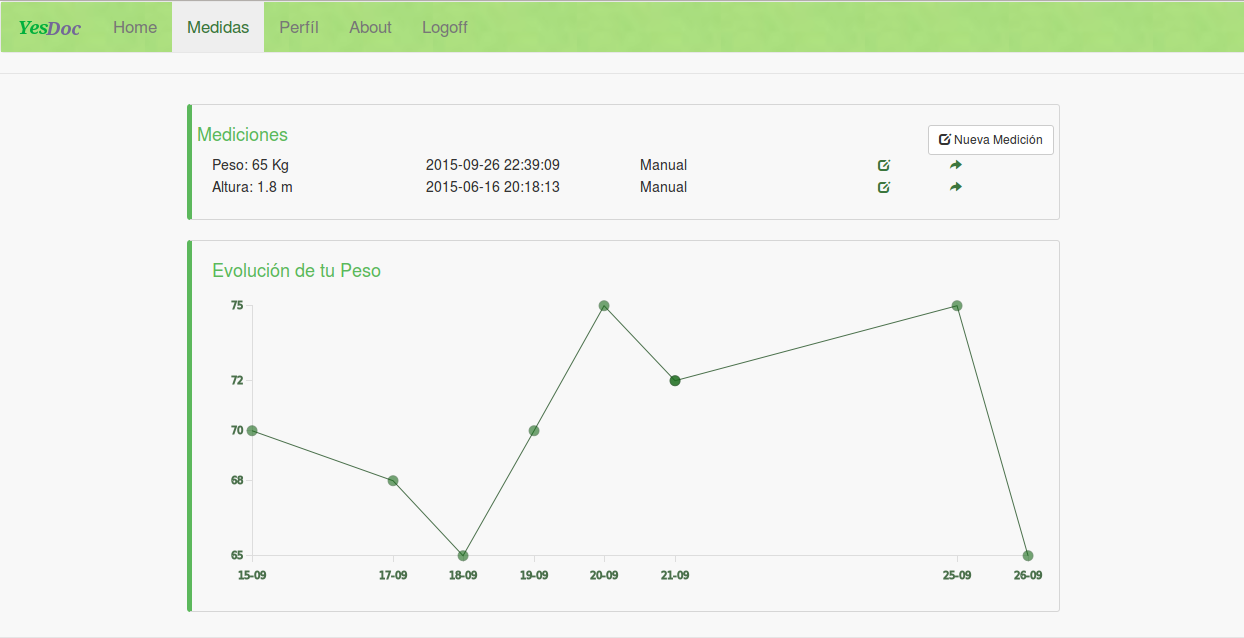
\includegraphics[width=.5\textwidth]{graph}
  \caption{Interfaz de usuario}
  \label{graph}
\end{figure}

\vspace{3mm}
\textbf{Discusión}

%(Times New Roman, 12, negrita) 
%Explica las relaciones, las tendencias, las posibles generalizaciones de los resultados observados, sin dejar de discutir aquellos resultados inesperados que invaliden total o parcialmente alguna de las hipótesis iniciales del trabajo. Debe poner los resultados en relación con los de otros trabajos e indicar las posibles aplicaciones (o implicaciones teóricas) de los resultados de la presente investigación. 

%%%%%%%
Nuestro trabajo se somete a discusión pública a través de la liberación de código en GitHub, para que todos aquellos interesados en el proyecto puedan realizar su aporte y transmitir sus inquietudes.
%A lo largo del desarrollo del proyecto nos encontramos con dificultades técnicas que fueron necesarias salvar con mayor investigación 
Uno de los mayores problemas a afrontar es la de conseguir universalizar los tipos de mediciones ya que actualmente no existe un estándar universal seguido por todas las instituciones, para resolver este problema fue necesario implementar el sistema de una forma totalmente flexible, capaz de adaptarse a los cambios y a las necesidades de cada una de las instituciones responsables de realizar la carga de los análisis.

El mayor impacto en la comunidad que ofrece YesDoc es la posibilidad de recibir los resultados de los análisis de cualquier institución en su propia plataforma.

% Esto de abajo sería para hablar un poco sobre resultados inesperados y tendencia.
%El hecho de que nuestro país siga un camino que lleve a la centralización de la información salud digitalizada en una entidad específicamente creada para ello podría invalidar parcialmente nuestra premisa de solucionar los problemas de unificación y centralización aunque no totalmente ya que dado el caso, esta entidad presentaría la información desde la perspectiva que siguen hospitales y centros médicos por lo que no anularía nuestras premisas de brindar una solución centrada en el paciente y que modifique la forma en que se comunican paciente y médico.
%Por otro lado vemos que nuestra solución presenta un gran potencial y  puede llegar a ser repetida por distintos países alrededor del mundo y hasta adoptada como de facto por sus habitantes .
%%%%%%%

\vspace{3mm}
\textbf{Conclusión}

%(Times New Roman, 12, negrita) 
%La conclusión debería ser la versión condensada de las secciones anteriores, presentando los resultados claves encontrados en el trabajo. Debería estar estrechamente relacionada con los objetivos que fueron presentados en la introducción. Muchas veces es, junto con el título, la parte mas leída y por lo tanto debe ser de comprensión fácil y exacta. 
YesDoc busca facilitarle la vida a todas aquellas personas que forman parte de las actividades relacionadas al cuidado de su salud, permitiéndole una comunicación fluida y cercana medico-paciente, un control detallado de su historial médico y principalmente la posibilidad de poder recibir  los resultado de sus análisis en su cuenta de YesDoc desde su celular o su computadora.

\vspace{3mm}
{\chico \textbf{Referencias}}

{\chico
%(Times New Roman, 10, negrita). 
%Documentación y bibliografía utilizada. Todas las publicaciones citadas deberán incluirse en la lista de referencias. La numeración será secuencial y estará entre corchetes: [1]. 

\nocite{*}
\printbibliography[
heading=bibintoc
]
}

\end{document}